\documentclass[10pt,a4paper]{article}
\usepackage[latin1]{inputenc}
\usepackage{amsmath}
\usepackage{amsfonts}
\usepackage{amssymb}
\usepackage{subfig}
\usepackage{graphicx}
\usepackage{tikz}
\usetikzlibrary{automata,positioning}

\usepackage[backend=bibtex]{biblatex} \addbibresource{ref.bib}

\author{\textsc{Regan Koopmans, 15043143}}
\title{\textsc{COS 314 - Assignment 1}}

\begin{document}

	\maketitle

		\section{Intelligence} \subsection{Origins} The word \textsl{intelligence}
		derives from the Latin word \textsl{intelligere}, meaning \textsl{to
		understand} \cite{etymonline2017}. The word is generally accepted to mean
		the capacity for reasoning, decision-making and problem solving.

			\subsection{Meaning in Personal Opinion}

				In my opinion, intelligence is the ability for some agent to comprehend
				the significance of its actions in the external world, with some
				predictions of its effects. In other words, I believe that intelligence
				is synonymous with some \textsl{internal model of reality}.

				This model, which is either built from experience or from inherent
				instinct or programming, has simple rules that can be used to
				extrapolate outcomes arbitrarily (within the limits of the model and the
				agent's computational capacity). The act of learning implies adding to
				this model. For illustration of this idea we can look at animals: \\\\
				Simple creatures, such as star-fish, survive completely on instinct.
				These animals can thus be described entirely by static physical and
				chemical processes. In this way, we can imagine these animals like any
				other natural system, such as the weather or rock formations. These
				animals are \textsl{alive}, but are not \textsl{intelligent}, and exist
				on predictable chemical rules.

				Contrast this to a crow, which has been shown to use tools to obtain
				food \cites{atlantic2017}. This behaviour is fundamentally different
				from that of the star-fish. The crow, like us, has the ability to see a
				desired outcome and design (possibly new) steps to achieve that goal.
				Specifically: \medskip \[ \text{\large Physical
				outcome}\rightarrow\text{\large Access to food}\rightarrow\text{\large
				Survival} \] Unlike the star-fish, the actions of the crow are
				\textbf{motivated}, \textbf{calculated} and \textbf{premeditated}. This
				is the defining feature between the two animals. Collectively we may
				call this property \textsl{intelligence}. Other characteristics we
				attribute to intelligence (such as self-awareness, reasoning and complex
				decision-making) are easily explained by this essential difference.
				Indeed, it is precisely for this distinction that these higher-order
				mental activities become useful to a living creature. Simple creatures
				still thrive without intelligence, and hence stay simple.

				Intelligent entities can evaluate situations which they have not
				directly experienced, through using aggregated knowledge from other
				experiences to form new assumptions about their environment. We
				recognise this ability as that of deduction. \\\\ This is the condition
				of individual intelligence, however another common form of intelligence
				exists: \textsl{group intelligence}, also known as \textsl{collective
				intelligence} or \textsl{swarm intelligence}. This is when many agents
				come together, and their collective actions solve some problem or task
				that is important to all of them. This behaviour is seen in both simpler
				animals (ants in an ant colony) and in complex/intelligent animals
				(dolphins hunting a school of fish). Through working together, creatures
				like ants can perform complex search algorithms and maintain adaptive
				transport routes, and dolphins can hunt large amounts of fish, with
				\textbf{proficiencies far beyond that of the individual}. \\\\ This is
				of course intelligence in a more \textsl{abstract form}, but as we
				investigate we discover it is the same intelligence as described for the
				individual, but simply \textbf{executed in distributed fashion}. The
				group has a collective awareness of the environment. The group will make
				decisions as a group, through the aid of some communication medium
				(sounds for dolphins, pheromones for ants). The animals can connect
				cooperation with mutual success (and of course humans do this too). One
				might say that these groups are greater than the sum of their parts. \\\\
				Intelligence is closely linked to perception. A larger perception
				implies a more comprehensive model of the environment. The more nuanced
				the internal model, the more varied the expected outcomes become, and
				hence give rise to a greater capacity for decision-making. Chess is a
				more intelligent game than Checkers, simply by the fact that there is
				more information in any given state of a chessboard, than that of a
				checkers board. Thus, an intelligent entity that wants to play chess
				proficiently must first perceive the significance of the pieces and the
				rules. Any ability beyond this comes from the agent's capacity to
				evaluate board states, and extrapolate these forward, directing to a
				desired outcome of their choosing. This is what a decision fundamentally
				is. Since energy is a scarce commodity in nature, some heuristic for
				solving problems is usually observed in biology. It is unlikely that
				evolution would ever produce an animal to play perfect Chess. \\\\ It is
				still a matter of debate whether intelligent creatures are deterministic
				in the same way bacteria and parasites are. It may be the case that
				complexity is the only factor that separates the star-fish from the
				crow. Of course we would like to think that intelligent creatures such
				as us actually make decisions, and are not inherently predictable. These
				concerns inevitably link to questions of the existence of free-will and
				the true nature of conciousness. Such philosophical questions are beyond
				the scope of this discussion, but I believe that I have sufficiently
				illustrated why I feel that intelligence is so closely tied to an
				internal representation of reality, whether held by the group or the
				individual.

		\pagebreak \section{Artificial Intelligence} \subsection{Origins} The term
		\textsl{Artificial Intelligence} was coined by John McCarthy in 1955
		\cite{intel}. The phrase is generally accepted to mean synthetic creations
		(particularly software) that demonstrate reasoning capacity comparable or
		similar in nature to that of humans.

			\subsection{Meaning in Personal Opinion}

				As described in \textsc{Section 1 - Intelligence}, I believe that
				intelligence is best described as a sandbox model of reality that an
				agent can use to evaluate scenarios in which they have a desired
				outcome. Hence I am of the opinion that we can make machines intelligent
				in the same manner that humans are, assuming a sufficient model and
				adequate processing. In most applications of Artificial Intelligence we
				have the following:

				\begin{itemize} \item a value to optimize or a task to complete. \item
				features, methods,  or ways in which a strategy might be modified. \item
				feedback, in the form of some model (typically number of successes
				versus failures in environment). \end{itemize}

				With these conditions, and sufficient data/time to iterate, many tasks
				that we deem intelligent (image recognition, language-processing and
				language comprehension), have been effectively simulated on computers. \\\\
				Therefore, I personally define artificial intelligence, in its broadest
				terms, as the creation of systems (whether physical or in software) that
				can \textsl{make calculated decisions}, based on one or more
				\textsl{desired criteria}, with some awareness of the decisions'
				probable outcomes. These expectations may be developed by machine
				learning, or through direct input of the programmer.

			\subsection{Main Purpose of The Field}

				Artificial Intelligence is primarily concerned with creating programs
				and machines that can reason with similar faculties as humans, in the
				aim of solving complex problems that traditional empirical programming
				paradigms struggle to solve. To this end, Artificial Intelligence is a
				tool which humans can use to vastly extend their problem-solving reach,
				and someday abstract general reasoning into mechanical processes.
				Artificial Intelligence allows us to imbue environments with intelligent
				devices, and thus live in a world that is more engaging, dynamic and
				responsive. \\\\ Artificial Intelligence enables other fields of study
				to grow in new directions and in faster rates. Artificial Intelligence
				can be taught to evaluate the validity of mathematical propositions in
				formal proofs \cite{atp}, which accelerates mathematical research. In
				medical research, Artificial Intelligence can estimate side effects of
				new medicines, and help doctors identify diseases and suggest treatment
				\cite{cancer}, all of which directly equates to helping human life.
				Artificial Intelligence can identify inefficiencies in man-made systems,
				and through doing so help us create smarter cities, smarter homes and
				better tools. \\\\ A large section of Artificial Intelligence involves
				the automation of tasks that were previously fulfilled by humans. Of
				course this raises a lot of concern among the general populace. However,
				we must ask ourselves whether the jobs that Artificial Intelligence
				automates are worth preserving. Menial jobs such as those in transport,
				logistics and record-keeping do not inspire the best of human creativity
				and innovation. The jobs that require the most humanity are the ones
				that survive, and are expected to survive long into the future. \\\\ A
				bi-product of these studies is further understanding in the cognitive
				process in biological animals, such as humans. Artificial Intelligence
				can help us deliberate on important questions in biology and
				neuroscience. Such investigations include whether conciousness is an
				emergent property (whether self-awareness simply falls out of mechanical
				structures like the brain), and the computational limits of the human
				mind. Further, Artificial Intelligence gives us new insight into the
				nature of intelligence. \textsl{Biological intelligence}, the
				intelligence that we are familiar with, is only an infinitesimally small
				fraction of all possible intelligences. This fact means that through
				artificial intelligence we can explore realms of intelligence foreign to
				our own. Summarised:

				\medskip \[ \text{\{Human Intelligence\}}\subset\text{\{Known
				Intelligences\}}\subset\text{\{All Possible Intelligences\}} \]

			\subsection{Contemporary Success in Real World}

				Recently (October 2016), the mining firm Rio Tinto deployed a fleet of
				69 self-driving industrial vehicles, to haul minerals for a mine in
				Pilbara, Western Australia. This is only the latest addition to this
				mine, which also features autonomous trains and drills. Andrew Harding,
				their iron ore chief executive said,

				\begin{center} \textsl{``Our autonomous fleet outperforms the named
				fleet by 12 per cent.''	} \end{center}

				 These machines can operate at all-hours, every day of the week, and are
				 monitored remotely more than a thousand kilometres away. The mine can
				 operate with \textsl{no humans on site}. This demonstrates that while
				 it may take a few more years for self-driving cars to achieve
				 mass-adoption in the main-stream, their deployment in industry is
				 already in progress. This shows that the software controlling these
				 machines has reached a proficiency that meets or exceed a humans', with
				 regards to the scope of the problem. \textbf{It is now in the financial
				 interest of industrial companies to utilise intelligent systems}. This
				 is a massive milestone for Artificial Intelligence.

		\pagebreak \section{Life}

			\subsection{Origins}

				The word \textsl{life} comes from Old English. It is most likely
				Germanic in origin, and has kept its original meaning through history
				\cites{etymonline2017}. Life is a fundamental concept for mankind (for
				obvious reasons), and features heavily in religion, ceremony and human
				experience.

			\subsection{Meaning in Personal Opinion}

				Life is a very alluding concept. Although living matter conforms to the
				same physical laws as most other matter, it does not initially appear to
				behave like any familiar substance. We are often told that ``nature
				takes the path of least resistance", but life seems contrary to this
				rule. Life feels unnecessary, perhaps even superfluous, in comparison to
				the stubborn, persistent processes in inorganic nature (think weather
				systems; movement of tectonic plates). \\\\ Physics, in our
				understanding, ``wants" to increase entropy and homoeostasis until
				energy is evenly dispersed across the universe. So why then, have living
				things arisen to essentially become sinks of energy? Living beings hoard
				energy as much as they can, and use it far slower than a fire might. On
				face value, life does not quite fit in. There are more efficient ways to
				disperse energy than life. I believe this is one of the major obstacles
				of studying life, because it already feels an incorrect act to try and
				harmonize life with non-life. This dichotomy gives life a mystical
				quality, and it may be more profound that life may not exist for a
				reason, than if it did. Regardless of the purpose of life, life exists,
				and below I have tried to summarise my own opinion on a definition: \\\\
				There are formal biological definitions of life. I feel that the
				measures used to describe life in biology are accurate in identifying
				life, but not necessarily in defining life.  In my opinion, life as we
				know it is an abstract concept describing \textbf{regular patterns in
				carbon-based molecules}. As minerals and crystals are the regular forms
				of atoms, so life (in its denominations) is the regular form of
				primordial carbon substances through time. Living things take in raw
				materials, and use these to build regular structures, as prescribed by
				DNA, and spawn new structures. Living creatures are also \textsl{regular
				in ``time"}, in that life forms will generally be born, mature, and die
				in repeated patterns through generations.

				One can try to perceive life almost as a stalactite, growing from the
				floor of a cave. Given enough time and resources (calcium rich water
				dripping from the ceiling), the stalactite will grow continuously. The
				stalactite may change course to accommodate changes in the water supply
				(evolution in the analogy). Changes in the cave topology may permit of
				forbid certain stalactites, and equally growth in stalactites will
				change the shape of the cave. So we have this inanimate, but
				``symbiotic" relationship: \bigskip \begin{center}

					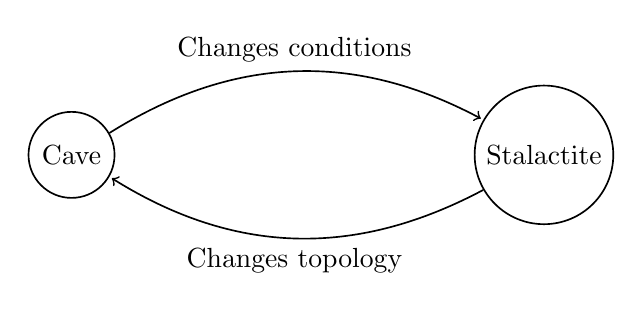
\begin{tikzpicture}[shorten >=1pt,node distance=6cm,on grid,
					auto,semithick] \node[state] (c) [] {Cave}; \node[state] (s) [right=of
					c] {Stalactite}; \path [->] (c) edge[bend left] node
					[pos=0.5,above]{Changes conditions} (s) (s) edge[bend left] node
					[below]{Changes topology} (c);

					\end{tikzpicture} \end{center} \bigskip This concept links closely to
					life, which is shaped by it's environment (via evolution and natural
					selection), and in turn the environment is modified by the presence of
					life. When thought about globally, it is inevitable that these living
					systems would result from inanimate processes. Non-living substances
					stay as there are (with a non-zero chance of becoming ``living"), and
					living things continue to live, or proliferate in reproduction. There
					is an implicit ``pressure" for life to emerge from the inanimate. It
					is only the fact that living systems ensure their own survival, that
					separates coral growing in a reef from a stalactite growing in a cave. \\\\
					This may seem a bit of a stretched, perhaps sensationalist idea.
					\textbf{My goal is not to equate static minerals with living beings},
					but rather to demonstrate that they are both representative of
					repetitive structure, and both manifestations of ideas of symmetry and
					pattern. This is done to try harmonise living things with the rest of
					the natural world, which of course seems so fundamentally different.
					The diagrams below perhaps illustrates my point better: \\\\
					\begin{figure}[h] \centering \subfloat[Shelled sea animals
					\cite{Sea}]{{\includegraphics[width=4cm]{animals} }} \qquad
					\subfloat[Crystallized minerals
					\cite{Crystal}]{{\includegraphics[width=5cm]{crystals} }}
					\caption{Similarities of crystalline and biological structures.}
					\label{fig:example} \end{figure}

		\pagebreak \section{Artificial Life}

			\subsection{Origins}

				The term \textsl{Artificial Life} was coined by the theoretical
				biologist Christopher Langton in 1986 \cite{artlife}. It is generally
				regarded to describe a field of study that researches the creation of
				life via synthetic means, whether it be robotic, bio-chemical or
				completely simulated in software.

			\subsection{Meaning in Personal Opinion}

				In my opinion, Artificial Life is any man-made system that performs or
				simulates most, if not all, of the traits commonly associated with
				biological life. This includes (but is not limited to):
				Consumption/processing of energy, Growth, Reproduction and an implicit
				need for self-protection \cite{cfl}. Artificial Life can also include
				subsystems of life, in which one crucial aspect of some life-form is
				isolated and studied in depth. Further, Artificial Life is any
				biological life that is created synthetically, and cannot be observed in
				undisturbed nature.

			\subsection{Main Purpose of Field}

				Artificial Life is concerned with, among other things, using nature as
				inspiration to design \textsl{better machines}, more \textsl{organic
				software systems}, and more \textsl{sophisticated bio-chemical
				solutions} to modern problems. Practical applications of this field
				include creating robots that have better kinetic abilities and
				proficiency through emulating nature \cite{boston}. In software,
				\textsl{artificial immune systems} help maintain the security of a
				network by copying behaviours seen in biological immune systems
				\cite{immune}. In agriculture and medicine, artificial life is being
				tested and used as delivery mechanisms for pesticides and medication
				\cite{geneng}. \\\\ Artificial Life complements the field of Artificial
				Intelligence, particularly in applications of \textsl{particle swarm
				optimization} (PSO) \cite{pos}, in which simple agents form to find some
				optima in a system, by emulating the movement of flocks of birds and
				insects. Similarly, evolutionary and genetic algorithms emulate
				evolutions with possible solutions to problems as ``creatures", and
				based on their success will determine the proliferation of that strategy
				in the next ``generation" of algorithms. This allows us to ``grow"
				algorithmic solutions bottom-up. Many of these solutions are new to
				humans, because this evolutionary method has no pre-conceived bias to
				any particular form of problem solving, except to avoid those that do
				not solve the problem. \\\\ By studying artificial life, we may also
				learn the probable origins of life on Earth, and discover the likelihood
				of life being a spontaneous process. With the help of genetic and
				evolutionary algorithms, we can begin to observe how evolution works in
				repeatable and controlled simulations. This synthetic environment
				(whether digital or natural), allows biologists to explore foreign forms
				of life, new biological processes and repeatable biological outcomes
				that may be yet unknown to mankind. \\\\ Artificial Life is also
				\textsl{philosophically} significant, in that it seeks to determine
				whether life created or simulated by humans should be considered life in
				the same way that biological life in nature is regarded. This can be
				summarised in the question: Should artificial life receive animal
				rights? Or even further: should artificial life, of a sufficient
				complexity, receive \textsl{human} rights? This may sound ridiculous,
				but in these seminal times we do not yet know the limits of artificial
				perceptual existence. We do not know what an artificial lifeforms'
				capacity for suffering might be.

				Some individuals argue that biological life is bound by an ethereal
				soul, and hence it cannot be replicated or fully simulated. Artificial
				Life takes these arguments, as delicate at they may be to personal
				belief systems, and evaluates them in a non biased, constructive,
				scientific manner.

			\subsection{Contemporary Success in Real World}

				One of the most successful Artificial Life projects is called OpenWorm,
				which is ``the first comprehensive computational model of the
				\textsl{Caenorhabditis elegans}, a microscopic roundworm"
				\cite{openworm}. It is the first purely software based simulation of a
				natural animal.

				The creature in nature is only comprised of roughly a thousand cells,
				and only a few hundred neurons. This made the animal easy to fully
				simulate physically, chemically and electro-mechanically. The team
				working on this project are using a ``bottom up" approach, and are
				simulating physics to observe the emergent behaviour of this digital
				creature.

				The initial results of this project have proved very successful. All of
				the results are publicly available to any individual, and the software
				itself is open source, such that any other research team can conduct
				their own unprecedented investigations. This ``Open Science" approach
				means that this research has gotten to those who need it the most,
				accelerating development. The hope is that this work will someday lead
				to much larger simulations of more complex organisms.

		\pagebreak \printbibliography

\end{document}
